\documentclass[10pt,twocolumn,letterpaper]{article}

\usepackage{cvpr}
\usepackage{times}
\usepackage{epsfig}
\usepackage{graphicx}
\usepackage{amsmath}
\usepackage{amssymb}
\usepackage{newfloat}
\usepackage{float}
\graphicspath{{images/}}
\DeclareFloatingEnvironment[%
	fileext=los,
	name=Exhibit,
]{exhibit}


% Include other packages here, before hyperref.

% If you comment hyperref and then uncomment it, you should delete
% egpaper.aux before re-running latex.  (Or just hit 'q' on the first latex
% run, let it finish, and you should be clear).
\usepackage[breaklinks=true,bookmarks=false]{hyperref}

\cvprfinalcopy % *** Uncomment this line for the final submission

\def\cvprPaperID{****} % *** Enter the CVPR Paper ID here
\def\httilde{\mbox{\tt\raisebox{-.5ex}{\symbol{126}}}}

% Pages are numbered in submission mode, and unnumbered in camera-ready
%\ifcvprfinal\pagestyle{empty}\fi
\setcounter{page}{1}

\hypersetup{
    colorlinks=true,
    linkcolor=blue,
    filecolor=blue,      
    urlcolor=blue,
}
\begin{document}

%%%%%%%%% TITLE
\title{Deep Cooperative Neural Network (DeepCoNN) for Movie Rating Prediction}

\author{Colby Wise\\
Columbia University\\
{\tt\small cjw2165@columbia.edu}
\and
Michael Alvarino\\
Columbia University\\
{\tt\small maa2282@columbia.edu}
\and
Richard Dewey\\
Columbia University\\
{\tt\small rld2126@columbia.edu}
}

\maketitle
%\thispagestyle{empty}

%%%%%%%%% ABSTRACT
\begin{abstract}
   For our project we implemented the Deep Cooperative Neural Network (DeepCoNN) 
   architecture outlined in the arXiv working paper 
   "Joint Deep Modeling of Users and Items Using Reviews for Recommendation" 
   (Zheng, Noroozi, et. al. 2017) to predict user movie ratings from user review text data. 
   The DeepCoNN methodology models users and items jointly using review text in two cooperative neural networks.
   One network learns feature representations from groupings of users and their reviews, while the other learns
   features from items and user reviews; both networks share a final interaction layer. The following paper
   describes our implementation of DeepCoNN architecture using movie review data and presents 
   our results.
\end{abstract}
\ \newline
\href{https://github.com/michaelAlvarino/Deep-Learning}{Project GitHub Repository}

%%%%%%%%% BODY TEXT
\section{Introduction}

\par The literature on recommendation systems is deep and until recently has traditionally focused on well-known matrix factorization algorithms, such as collaborative filtering ($CF$), as popularized by Netflix and Spotify. Collaborative filtering is advantageous to other methods because it is relatively easy to implement and computationally efficient. On the other hand, the drawbacks of collaborative filtering in real-world applications lead to at times insurmountable challenges. To clarify, CF suffers from the "cold-start" problem in that it requires user ratings to make predictions. When users have no or limited prior ratings history relative to the total amount of items to rate this is called data \textit{sparsity}. For sparse user data it's difficult to accurately predict ratings/recommendations thus leading to poor model performance and generalization [9]. 

\par Recent breakthroughs in Deep Learning particularly in natural language modeling via convolutional neural networks ($CNN$) and recurrent networks ($RNN$) to capture complex feature interactions in textual data have lead recent recommendation systems ($RecSys$) research to begin to incorporate deep learning. CNN models [1] and RNNs [3] have shown the ability to help with the generalization problem and improve model accuracy in sparse data sets.

\subsection{Related Work}
Our experiments will focus on expanding the $DeepCoNN$ model thus our primary reference will be the original \textit{Joint Deep Modeling of Users and Items Using Reviews for Recommendation} paper. While the authors do not provide an open-source code repository on-line, after reaching out them via email they provided guidance on model replication. Additionally, we found a similar code base on-line that utilized video game review data [8]. Related papers we referenced for re-constructing $DeepCoNN$ are $DeepFM$ [4] which similar to our model, combines a form of matrix factorization to capture user/item interactions with a CNN architecture; $TransNets$ [3], which extends $DeepCoNN$ to examples where the users review is not available; and for background on factorization machines [2]. 

It should be noted that our original proposal was to replicate Google's \textit{Wide \& Deep} model [5]. We spent a considerable amount of time going down this path, but ultimately came to the conclusion that we could not source the high quality categorical data needed for training the wide part of the model. We decided to switch to the $DeepConn$ model due to it's greater relevancy to our data set despite the model being arguably more complex. 

%-------------------------------------------------------------------------
\section{Methodology}
This section outlines the methodology used in the project including an overview of the problem formulation, data set structure and processing, and details of model architecture.

\subsection{Problem Formulation}

\textit{In order to make better movie recommendations how can we more accurately predict a users rating for an unseen movie based on what the user has previously seen? Furthermore, can we improve generalization of our model when information on a users past movie ratings is limited by utilizing user review data?}\\

These two questions are the crux of our problem. Prior to deep learning, standard approaches for recommendation systems ($RecSys$) used collaborative filtering which relies on decomposing users, items (i.e. movies), and ratings into latent feature matrices. The interaction between users and items is captured by matrix multiplication of the weight matrices of these latent features. One common CF method includes using the cosine similarity measure between all pairs of movies that users have rated:\\

Where,
$m_{i}$ and $m_{j}$ refer to movie vectors of ratings of users who have rated both movies:

\begin{center}
\textbf{$cos(\theta)$} =
$\frac{\vec{m_{i}} \bullet \vec{m_{j}}}{||\vec{m_{i}}||_2 \times ||\vec{m_{j}}||_2}$
\end{center}

This yields a movie-to-movie similarity matrix of dimensions $M \times M$ with ones along the diagonal. Thus, the predicted rating for movie $m_{2}$ for $user_1$ would be calculated using similarity measures between ($m_2,m_1$) and ($m_2,m_3$) weighted by the respective ratings for $m_1$ and $m_3$. 

From the above formulation we can clearly see the major disadvantage of this approach: $sparsity$. When ratings are limited the movie-to-movie matrix is mainly zeros thus limiting predictive ability. Current research like $DeepCoNN$ have attempted to improve accuracy of sparse data by using text data that users write after watching movies. This text data is used as input for training neural networks and offers additional insights versus only numerical ratings.

The DeepCoNN model formulation that we'll focus on in this research uses two jointly modeled neural networks. The first network $Net_{i}$ uses all of the text reviews for a given user. The second network $Net_{p}$ uses all of the text reviews for a particular item (movie).

\subsection{Data Structure \& Processing}
The Amazon Instant Video Review 5-core data is a JSON file with nine values per entry of which we use:\\
\ \newline
 \hspace*{10mm}  \textbf{reviewerID} - user ID \\ 
 \hspace*{10mm}  \textbf{asin} - movie ID \\
 \hspace*{10mm}  \textbf{reviewText} - review text \\
 \hspace*{10mm}  \textbf{overall} - movie rating \\

Word embeddings map words our review text to $n$-dimensional numerical vectors. The paper does not explicitly state a standard word embedding method i.e. (GloVe, Word2Vec, etc) thus we decided to use Global Vectors for Word Representation (GloVe.6B) 50-dimensional pre-trained embeddings [10]. The purpose of this is to capture text structure from the review data. With this in hand, we group reviews by user and by movie into two dictionaries such that each key in the dictionary is a unique reviewerID accompanied by a list of their text reviews. Using Keras each review is tokenized into separate lowercased words with all punctuation removed. Then we use our embedding mapper to transform all reviews into their embedding representation. We carry out the same procedure for movie review except this time grouping movies with all their respective reviews. Finally given review lengths typically differ, prior aggregating all user reviews and movie reviews into input matrices we pad (truncate) shorter (longer) reviews such that input matrices are equal in dimensions. 

\subsection{Architecture}
The architecture of DeepCoNN is depicted below and taken from the original research paper [1]. The model has two parallel neural networks joined in the last layer. One network for
users and one network for movies.\\
\ \newline
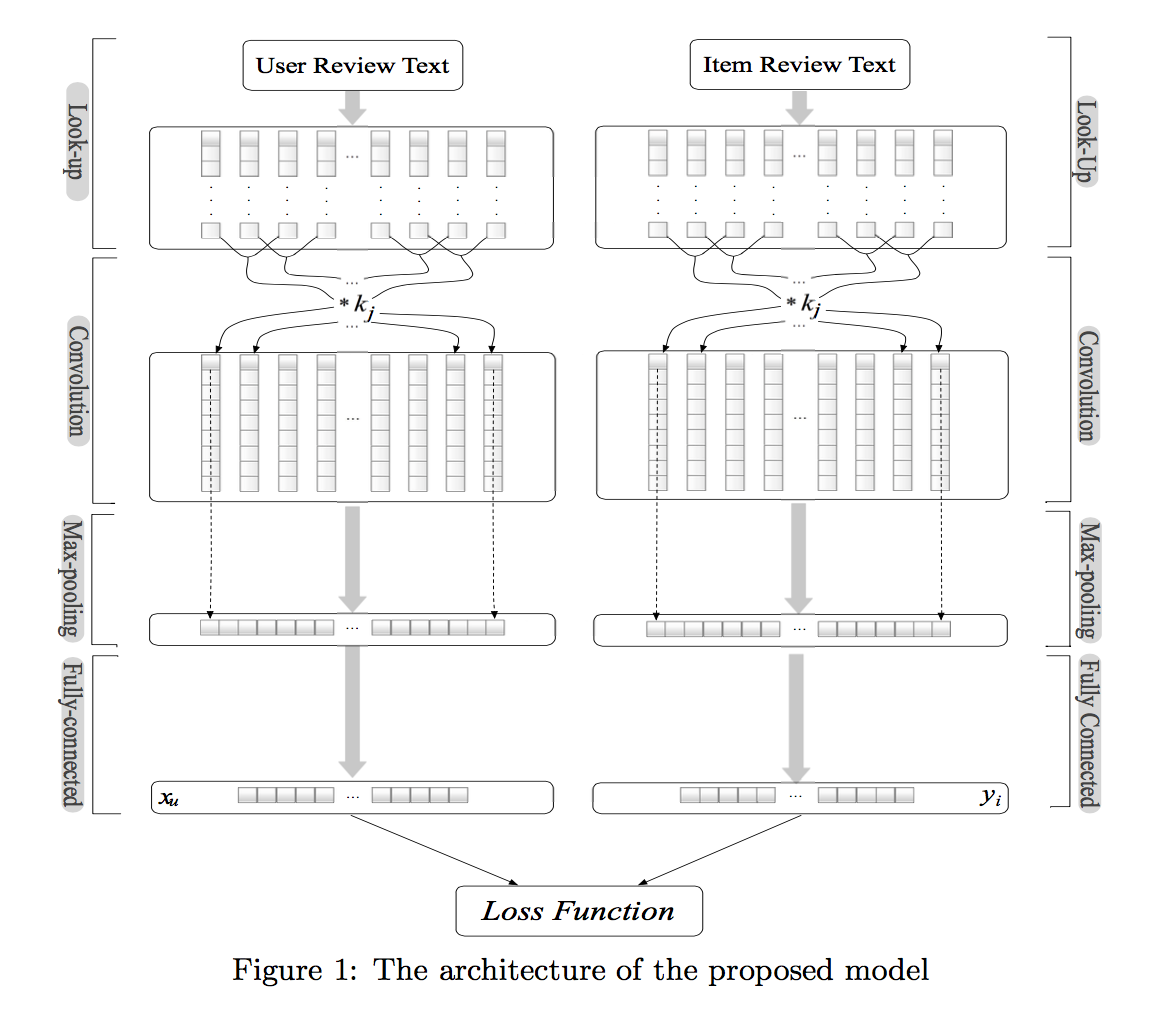
\includegraphics[scale=0.38]{DeepCoNN}

Note that in the original paper the first layer of the network is a "lookup" layer that transforms review text into embeddings. As discussed above, we create embedding prior to feeding into the network thus we omit a explicit "lookup" layer. Since the embedding layer uses pre-trained embedding and this is non-trainable our method is similar. The next layers are standard to CNN layers, however the exact number of convolutional layers is missing from the paper. For our preliminary implementation we used (per network): \\

\begin{enumerate}
\item CNN Layers: 1 \\
    \hspace*{5mm} Filters: 2 \\
    \hspace*{5mm} Kernel Size: 8 \\
    \hspace*{5mm} Strides: 6 \\
    \hspace*{5mm} Activation: ReLU 
\item Max Pooling Layers: 1
\item Flattened Layers: 1
\item Fully-Connected Layers: 1
\end{enumerate}

To train two networks simultaneously using a single loss function, the paper combines the outputs of both networks by concatenation. From here the interaction of user review features with movie review features is done via a \textit{factorization machine} of which the details are not provided. After contacting the authors, we were told that taking the dot product of the output from the fully connected layers of $Net_{u}$ and $Net_{i}$ should closely resemble the factorization machine approach. Optimization is done via $Adam$, which is an adaptive version of gradient descent that controls the step size with respect to the absolute value of the gradient. The paper did not use regularization.

%\section{Experiments}

\subsection{Results}

Our preliminary work consisted of reconstructing aspects of the codebase for DeepCoNN to model text review data for movie rating prediction as discussed above. We then built two new architectures, an LSTM network and a GRU network. We also experimented with various forms of regularization, tested different word embeddings and hyperparameters.

For a baseline comparison we used Amazon Music Instruments data set and obtained similar mean squared error ($MSE$) loss metrics as the paper's findings. The baseline used the \textit{dot product} interaction layer described in the paper. Table 1 below provides specifics on the training/test data split and key data metrics. While Table 2 shows the training time and $MSE$ loss of our implementation of DeepCoNN.

Our first innovation beyond the described DeepCoNN model involved testing two new network architectures, an LSTM network and a GRU network. Both the LSTM and GRU networks showed superior performance on the accuracy measure, but were much slower to train. See Exhibit 3 for training accuracies and training times of the architectures in comparison with the DeepCoNN network.  In addition to these architectures, we experimented with different hyperparameters, but found the tuning only led to very marginal differences in our results and so we decided to the standard parameter setting outlined in exhibit 4. 

After implementing our new architectures we sought improvement by testing the performance of GloVe 100 embeddings. This increases the token size from roughly 400,000 for GloVe 50 to roughly 1.5m tokens. Not surprisingly this increased token size led to improved performance as noted in the Exhibit 4 below. We also experimented with untrained embedding and the various review length limits for training. Neither of these two had a meaningful impact on our results.  

Finally we experimented with various forms of regularization. For the LSTM and GRU architectures we used a recurrent dropout (removing layers) and standard dropout of masking the activation of some nodes. For the DeepCoNN network we used l1 and l2 regularization as well as standard dropout, neither of which were explored by the authors. The results of our regularization are found in the Exhibit 5 below. Regularization improved most models by a marginal amount.  


\section{Conclusion}

The DeepCoNN model represents a step forward in recommendation systems and the typical collaborative and content-based filtering systems that were traditionally used. This was confirmed by our research into predicting movie rankings. Our research indicates that the DeepCoNN model can be incrementally improved by utilizing different word embedding structures and regularization. Moreover significant improvement to accuracy are available for a move into different architectures. The tradeoff with these new architectures is that they are significantly more complex and more time consuming to train. Practitioners may well continue to focus on collaborative filtering and the standard DeepCoNN model, but with improved compute power, these new architectures should gain acceptance and warrant further research.  

\begin{exhibit}
\begin{center}
{\small
\begin{tabular}{l|cccc}
\hline
%Category & Experiment Summary  \\ \hline
 & Training Time (seconds) & MSE Loss \\
\hline
DeepCoNN-DP & 262 & 1.0954   \\
LSTM & 2095 & .9835  \\
GRU & 5273 & 1.0532  \\
\hline
\end{tabular}
}
\end{center}
\caption{Results - Model Comparison}
\end{exhibit}


\begin{exhibit}
\begin{center}
{\small
\begin{tabular}{l|cccccc}
\hline
%Category & Experiment Summary  \\ \hline
 & Input Layers & Embedding Layers & Regularization & Dropout  \\
\hline
DC-DP & 64 & 50d and 100d & N/A & .1  \\
LSTM & 64 \& 32 & 50d and 100d & Recurrent & .1 \\
GRU & 64 \& 32 & 50d and 100d  & Recurrent & .1 \\
\hline
\end{tabular}
}
\end{center}
\caption{Architecture Overview}
\end{exhibit}






The DeepCoNN model shows superior performance over standard collaborative filtering techniques and the Wide and Deep model proposed by Google researchers. Our research into other architectures and regularization methods show that further improvements to DeepCoNN are available.   

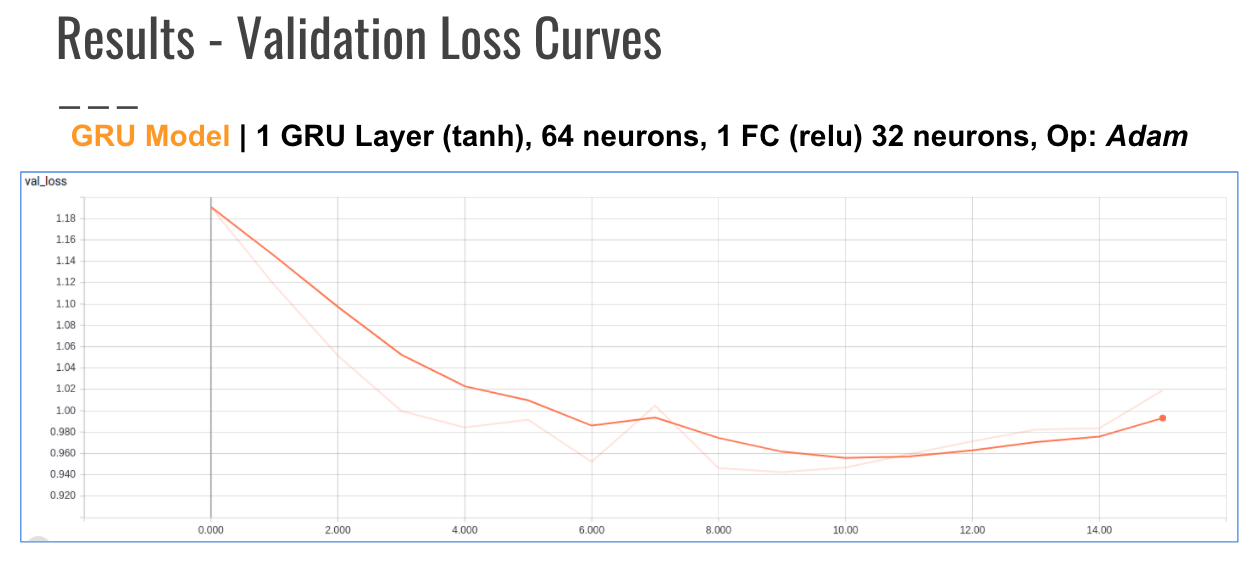
\includegraphics[scale=0.38]{Loss_Graph.png}


\begin{exhibit}
\begin{center}
{\small
\begin{tabular}{l|ccccccc}
\hline
%Category & Experiment Summary  \\ \hline
 & \# Reviews & \# Users & \# Movies & Training\% & Test\% \\
\hline
Data & 18,563  & 5033 & 1685 & 90\% & 10\%  \\
\hline
\end{tabular}
}
\end{center}
\caption{Amazon Instant Video Dataset Overview}
\end{exhibit}

%Exhibit2
\begin{exhibit}
\begin{center}
{\small
\begin{tabular}{l|ccccccc}
\hline
%Category & Experiment Summary  \\ \hline
Model & MSE & Training Time & Epochs \\
\hline
DeepCoNN-DP & 1.2645 & 10 min & 20  \\
\hline
\end{tabular}
}
\end{center}
\caption{DeepCoNN-DP Initial Results}
\end{exhibit}


\section{References}

[1] Zheng, Lei, Noroozi, Vahid and Yu, Philip. Joint Deep Modeling of Users
 and Items Using Reviews for Recommendations. arXiv working paper, June 2017

[2] Rendle, Steffan. Factorization Machines. ICDM 2010

[3] Catherine, Rose and Cohen, William. TransNets: Learning to Transform
for Recommendation. arXiv working paper, June 2017

[4] Huifeng Guo, Ruiming Tang, Yunming Ye, Zhenguo Li, and Xiuqiang He
DeepFM: A Factorization-Machine based Neural Network for CTR Prediction
arXiv working paper, March 2017

[5] Heng-Tze Cheng, Levent Koc, Jeremiah Harmsen, Tal Shaked, Tushar Chandra, Hrishi Aradhye, Glen Anderson, Greg Corrado, Wei Chai, Mustafa Ispir, Rohan Anil, Zakaria Haque, Lichan Hong, Vihan Jain, Xiaobing Liu, and Hemal Shah.
Wide \& Deep Learning for Recommender Systems. arXiv working paper, June 2016

[6] A. Baylen. Github Repo $Uifud$
https://github.com/Praznat/uifud
As of 11/27/17 

[7] J.Pennington, R. Socher, C.Manning. Global Vectors for Word Representation 
version: 6B.50d.txt. https://nlp.stanford.edu/projects/glove/ 
Available as of 11/27/17 

[8] Image-based recommendations on styles and substitutes
J. McAuley, C. Targett, J. Shi, A. van den Hengel
SIGIR, 2015

[9] Balakrishnan Anusha, Dixit Kalpit. DeepPlaylist: Using Recurrent Neural Networks to
Predict Song Similarity. semanticscholars.org 


\end{document}


Our first development phase of the project the \textit{shared layer} between the user network and the movie network was done by a dot product ($DP$) of the outputs of both networks. This method is straightforward to implement, but suffers from the fact that it does not capture higher order interactions between features. To this point, in addition to this $DP$ share layer the paper tests a factorization machine ($FM$) layer showing that \textit{DeepCoNN-FM} outperforms \textit{DeepCoNN-DP} empirically. However the authors provide no specifics on the implementation of this factorization machine. In the second phase we implemented a factorization machine as well and, like the authors, realized improved prediction accuracies. 


%For our final project we will try to implement a factorization machine by utilizing some of the additional resource papers mentioned.

%Furthermore, we also intended to test other hyperparameter settings and different architectures that empirically have shown good results when working with text data such as %LSTMs. During this process we will also experiment with adding regularization to the model given the original paper does not mention this.  

